\section {Примеры}

\subsection * {Задача 1}
Найти все значения параметра $p$, при которых квадратное уравнение
$(p - 1) \cdot x^2 - 2p \cdot x + (p + 3) = 0$ имеет ровно два корня на луче $[0, +\infty)$.

\subsection * {Решение}
Для начала рассмотрим особый случай. Им является попадание одного из корней в точку $x = 0$ при
нахождении второго корня на луче $[0, +\infty)$. Чтобы учесть этот случай, решим уравнение
$f(0) = p + 3 = 0$ и проверим, попадает ли второй корень на луч $[0, +\infty)$. Подставляем
значение параметра $p = -3$ в исходное уравнение и находим его корни:
\begin {equation*}
    -4x^2 + 6x = 0
    \quad\longrightarrow\quad
    \left[
        \begin {aligned}
            x_1 &= 0
            \\
            x_2 &= 1.5
        \end {aligned}
    \right.
\end {equation*}
корень $x_2 > 0$, следовательно, значение параметра $p = -3$ подходит.\\

Теперь можно рассмотреть общий случай. Один из корней уравнения должен находиться на луче
$[0, +\infty)$, а второй лежать левее точки $x = 0$.

\begin {figure} [h]
    \begin {minipage} [t] {\linewidth}
        \centering
        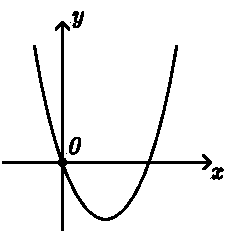
\includegraphics [width=0.3\linewidth] {image/image_16.pdf}
    \end {minipage}
\end {figure}

Этим условиям удовлетворяет следующая система уравнений:
\begin {equation*}
    \begin {cases}
        D = p^2 - (p-1)(p+3)  > 0
        \\
        (p - 1) \cdot f(0) = (p-1)(p+3) > 0
        \\
        x_0 = \dfrac{p}{p-1} > 0
    \end {cases}
    \longrightarrow\quad
    \begin {cases}
        p \in (-\infty, 1.5)
        \\
        %p \in (-\infty, -3) \cup (1, +\infty)
        p \in \mathbb{R} \, \backslash \, [-3, 1]
        \\
        %p \in (-\infty, 0) \cup (1, +\infty)
        p \in \mathbb{R} \, \backslash \, [0, 1]
    \end {cases}
\end {equation*}
решаем её и находим значения параметра: $p \in (-\infty, -3) \cup (1, 1.5)$.

\subsection * {Ответ}
Объединяя множества значений параметра, полученные в особом и общем случаях, получаем ответ задачи:

\begin {equation*}
    \boxed{p \in (-\infty, -3] \cup (1, 1.5)}
\end {equation*}